%%%% début de la page

\renewcommand{\thesubsection}{\textcolor{red}{\Roman{section}.\arabic{subsection}}}
\renewcommand{\thesubsubsection}{\textcolor{red}{\Roman{section}.\arabic{subsection}.\alph{subsubsection}}}

\setcounter{section}{0}
\setcounter{document}{0}
\sndEnTeteTPQuatre

\begin{center}
\begin{mdframed}[style=titr, leftmargin=60pt, rightmargin=60pt, innertopmargin=7pt, innerbottommargin=7pt, innerrightmargin=8pt, innerleftmargin=8pt]

\begin{center}
\large{\textbf{TP 4 : Comment bien choisir la verrerie pour mesurer des volumes précis ?}}
\end{center}


\end{mdframed}
\end{center}

%\begin{tableauCompetences}
 %   ANA & Mesurer des volumes & & & &
    
%\end{tableauCompetences}

%%%% objectifs
\begin{tcolorbox}[colback=blue!5!white,colframe=blue!75!black,title=Objectifs de la séance :]
\begin{itemize}
    \item Mesurer des masses pour étudier la variabilité du volume mesuré par une pièce de verrerie
  %\item Choisir et utiliser la verrerie adaptée pour préparer une solution par dissolution
\end{itemize}
\end{tcolorbox}

%%%% contexte

\begin{tcolorbox}[colback=orange!5!white,colframe=orange!75!black,title= Scénario:]
Le laboratoire dispose de trois principales pièces de verrerie qu'on utilise couramment lors de manipulation complexe. Nommer ces trois verreries.
\begin{center}
    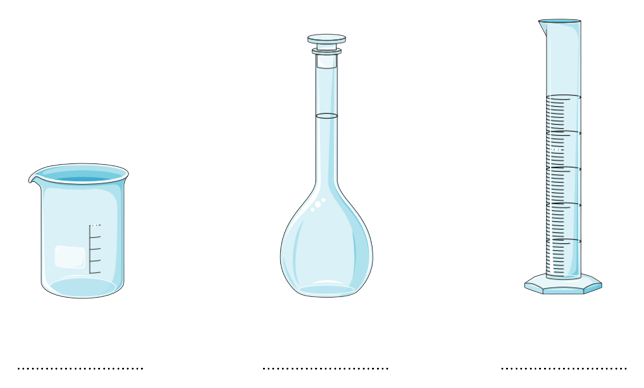
\includegraphics[scale=0.7]{Images/Verrerie_a_completer.png}
\end{center}
\problematique{On souhaite vérifier que la fiole jaugée est la pièce de verrerie la plus précise et la plus fidèle. Comment fait-on ?}
\end{tcolorbox}

\begin{tcolorbox}[colback=red!5!white,colframe=red!75!black,title= Consignes :]
\begin{itemize}
    \item Vous travaillez collaborativement par rangées de 2 binômes,
    \item Dans chaque binôme, nommer un responsable \og MES \fg : il aura la responsabilité de vérifier la bonne réalisation des mesures et de rentrer les valeurs expérimentales sur le fichier Excel du tableau. Nommer également un responsable \og COM \fg : il aura la responsabilité du compte-rendu et fera office de porte-parole du binôme,
    \item Faire attention à la verrerie lors de son utilisation,
    \item Respectez les consignes d'utilisation de la salle de chimie.
\end{itemize}

\end{tcolorbox}
\begin{mdframed}[style=autreexo]
\textbf{\bsc{Liste du matériel}}
\vspace{-0.5cm}
\begin{multicols}{2}
\begin{itemize}
    \item une balance, 
    \item un bécher de 50~mL
    \item un bécher de 100~mL,
    \item une fiole jaugée de 100~mL,
    \item une éprouvette graduée de 100~mL,
    \item une pipette plastique,
    \item une pissette d'eau distillée,
    \item un ordinateur avec le tableur Excel.    
\end{itemize}
\end{multicols}
\end{mdframed}

\newpage
%%%% documents
\begin{doc}{Lecture d'un volume sur la verrerie}

\begin{wrapfigure}{r}{0.3\textwidth}
\vspace{-2cm}
    \centering
      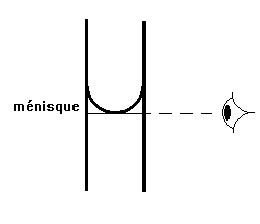
\includegraphics[width=0.27\textwidth]{Images/Lecture_Verrerie.png}
  \end{wrapfigure}
  Lorsqu'on verse un liquide dans une pièce de verrerie (éprouvette, tube à essai, etc), il se forme un ménisque qui va perturber la lecture du volume sur la verrerie. Pour lire le volume occupé par un liquide, il faut positionner son \oe il sur le bas du ménisque.
\end{doc}

%%%%
\begin{doc}{Protocole de remplissage d'une fiole jaugée}
  \label{doc:fiole_jaugee}
  \begin{center}
      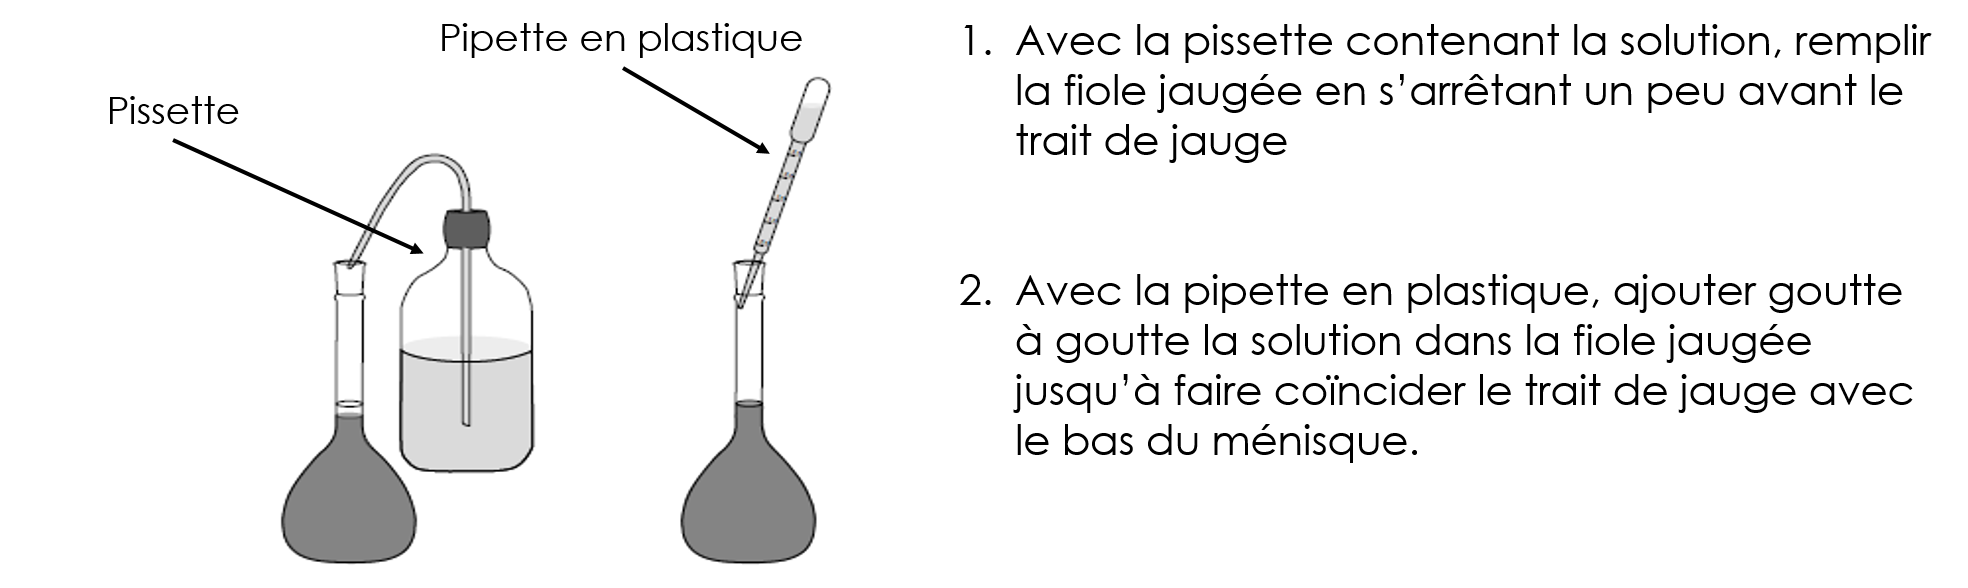
\includegraphics[scale=0.5]{Images/Protocole_fiolejaugee.png}
  \end{center}
\end{doc}

%%%%
\begin{large}
    \textbf{\textcolor{red}{\underline{Travail à réaliser :}}}
\end{large}

\question{Récupérer le fichier \og TP4Resultats.xlsx \fg~dans le dossier de votre classe sur l'ENT dans l'application \og Espace Documentaire \fg. }{~}{0}
\question{Comment réaliser la mesure d'un volume d'eau distillée avec une balance ? Vous écrirez le protocole expérimental sur votre compte-rendu \underline{avec la formule que vous utiliserez}.}{On connaît la masse volumique de l'eau $\rho_{eau}=\frac{m}{V}=1$~g.mL$^{-1}$. En pesant la masse d'eau contenue dans la verrerie (après avoir soustrait la masse de la verrerie bien sûr), on en déduit immédiatemement le volume d'eau}{0}

\question{Pour chaque type de verrerie, réaliser 3 fois la mesure d'un volume de 100~mL d'eau distillée. Compléter le tableau suivant avec vos résultats :
\begin{center}
    \begin{tabular}{|c|C{0.2}|C{0.2}|C{0.2}|}
    \hline
         Verrerie & Mesure n°1 & Mesure n°2 & Mesure n°3  \\
         \hline
         \cellcolor{blue!25} Bécher &   &  & \\
         \hline
         \cellcolor{blue!25} \'{E}prouvette graduée &   &   &\\ 
         \hline
         \cellcolor{blue!25} Fiole jaugée &   &   &\\
         \hline
    \end{tabular}
\end{center}}{Blabla}{0}

\question{Rentrer vos valeurs dans votre tableur Excel et dans celui du binôme de votre rangée.}{~}{0}
\question{Le responsable MES vient compléter avec ses mesures le tableau Excel au tableau.}{~}{0}
\question{Avec les fonctions MOYENNE et ECART-TYPE du tableur Excel, calculer la valeur moyenne et l'écart-type pour chaque verrerie.}{~}{0}
\question{Imprimer les graphiques de vos mesures pour chaque verrerie : sélectionner les 3 graphiques, cliquer sur Fichier-> Imprimer -> Aperçu avant impression.}{~}{0}
\question{Représenter la moyenne et l'écart-type sur vos graphiques.}{~}{0}
\question{A l'aide des moyennes et des écart-types, justifier quelle est la verrerie la plus précise.}{~}{0}